%++++++++++++++++++++++++++++++++++++++++
% Don't modify this section unless you know what you're doing!
\documentclass[letterpaper,12pt]{article}
\usepackage[T1]{fontenc}
\usepackage[utf8]{inputenc}
\usepackage[italian]{babel}
\usepackage{tabularx} % extra features for tabular environment
\usepackage{verbatim}
\usepackage{amsmath}  % improve math presentation
\usepackage{graphicx} % takes care of graphic including machinery
\usepackage[margin=1in,letterpaper]{geometry} % decreases margins
\usepackage{cite} % takes care of citations
\usepackage[final]{hyperref} % adds hyper links inside the generated pdf file
\DeclareGraphicsExtensions{.pdf}
\hypersetup{
    colorlinks=true,       % false: boxed links; true: colored links
    linkcolor=blue,        % color of internal links
    citecolor=blue,        % color of links to bibliography
    filecolor=magenta,     % color of file links
    urlcolor=blue         
}
%++++++++++++++++++++++++++++++++++++++++


\begin{document}

\title {Rheological measurements of non-newtonin liquids based on drop oscillation}
\author{A. Mischianti}
\date{Luglio 2020}
\maketitle



\section{Introduction}
Non-newtonian fluids exhibits a viscosity which varies with the shear stress. Everyday life examples of non-newtonian fluids include ketchup, toothpaste, paints, shampoos, blood, etc. Therefore, their rheological properties have a very important impact in many applications such as chemical industries, biological analysis, microfluidics, ink jet printing, fuel injection, etc. The rheological characterization is typically performed using commercial rheometers, which measure the fluid response to applied forces. These instruments present some restrictions in terms of minimal volume required for the analysis and, additionally, they are expensive. \\
A viable alternative is to use a single droplet ($\simeq \mu L$) deposited on a horizontal surface and subjected to an external mechanical stimulus. By analyzing the decay of the induced capillary modes it is possible to determine the liquid viscosity. This method allows to dramatically reduce the liquid volume and the costs required for the viscosity determination. \\
During the internship, the student will contribute to the development of the experimental setup needed for the rheological characterization, acquire some preliminary data and develop a program for the data analysis.\\

The activity will be divided in two parts: at first, the student will optimize the experimental protocol for acquiring the measurements in the lab (1-2 weeks expected); then, he/she will develop a customized software for analyzing the acquired data and discussing the results. \\
The second part of the activity does not require the presence in the lab. 
The student, assisted by a post-doc, will learn the basics of wetting and rheology, as well as how to assemble a customized experimental setup and data analysis program.
\subsection {Goals of the experience}
The goals of the experience are:

\section{Theory}
\subsection{Microfluidica}
La microfluidica è il settore scientifico che si occupa dello studio e della manipolazione di piccoli volumi di liquidi ($\mu L \ pL$), confinati su scale submillimetriche. In queste condizioni il comportamento di un fluido è radicalmente diverso da quello che esprime a volumi ordinari perché caratterizzato dai fenomeni interfacciali e viscosi: le forze capillari dominano la gravità (bassi numeri di Bond (Bo) - il rapporto tra la gravità e la tensione superficiale:  in un sistema microfluidico il numero di Bond sarà proporzionale a $10^{-12}$, essendo Bo molto piccolo, sono prevalenti le tensioni superficiali rispetto alla forza peso. Questo è uno dei principali motivi per cui, ad esempio, gli insetti riescono a "scalare i muri".) e i moti sono laminari (bassi numeri di Reynolds - Il numero di Reynolds rappresenta fisicamente il rapporto tra le forze d'inerzia e quelle viscose agenti su una particella fluida che si muove con velocità U all'interno dello stesso fluido). Alla microfluidica fanno capo un numero sempre crescente di tecnologie che trovano applicazione nella ricerca in fisica, microbiologia, chimica combinatoriale e medicina molecolare, oltre che in processi industriali e commerciali quali la stampa a getto d'inchiostro, lo spray coating o l'iniezione di combustibile. 


\subsection{Fluidi:Tensione superficiale e bagnabilità}
I fenomeni interfacciali acquisiscono importanza rispetto a quelli di volume a mano a mano che si riduce la dimensione degli oggetti considerati, poiché aumenta il rapporto superficie-volume. Per gocce liquide di alcuni microlitri è essenziale perciò considerare il ruolo predominante delle forze che si sviluppano a cavallo della pellicola superficie: le forze capillari. In presenza di una separazione tra due fluidi immiscibili (come ad esempio acqua e aria) le molecole poste all'interfaccia risentono di un sostanziale sbilanciamento di forze rispetto a quelle situate all'interno. Questo fatto, come noto, risiede nell'isotropia delle interazioni intra-molecolari (interazioni di Van der Waals, legami a idrogeno,...) nelle varie parti del fluido. Ove dette interazioni (solitamente attrattive) cessano di essere isotrope, cioè in prossimità della superficie di separazione, le molecole sono sottoposte ad una risultante diretta verso il bulk (gli atomi sulla superficie hano meno primi vicini, e tutti da un lato) e tendono perciò ad occupare la minima area compatibile con le condizioni al contorno. All'aumentare della superficie aumenta il numero di interazioni molecolari non bilanciate e quindi l'energia (libera) ad esse associata. Per espandere la superficie (A) è pertanto necessario fornire lavoro (W). \\
La tensione superficiale $\gamma$ rappresenta l'energia fornita dall'esterno per ottenere un aumento unitario della superficie dell'interfaccia, ossia 
\begin{equation}
	\gamma=(\frac{\partial G}{\partial A})_{T,p}
\end{equation}
ove T è la temperatura e p la pressione sul liquido. Equivalentemente, la tensione superficiale si può interpretare come la forza per unità di lunghezza L che il fluido esercita perpendicolarmente ad ogni sezione dell'interfaccia: 
\begin{equation}
\gamma=\frac{\partial F_{perp}}{\partial L}
\end{equation}
Questa forza, detta forza capillare, rende la pellicola superficiale una membrana tesa e ne stabilisce la geometria in ogni condizione di equilibrio. In virtù di ciò, evidentemente, una minuscola goccia liquida posta in aria, pendente da un ago oppure posta su di un piano (sessile) tenderà ad assumere una forma emisferica e vi si accosterà tanto più quanto più il contributo capillare domini su quello gravitazionale.\\
Al di sotto di una certa dimensione caratteristica, detta lunghezza di capillarità, definita come:
\begin{equation}
	\kappa^{-1}=\sqrt{\frac{\gamma}{g \rho}}
\end{equation}
 la forma di una goccia sessile dipende unicamente dall'equilibrio fra le tensioni cui sono soggette le tre interfacce esistenti: quella tra substrato solido e liquido ($\gamma_{SL}$), quella tra solido e ambiente gassoso ($\gamma_{SG}$) e la tensione superficiale del liquido in aria ($\gamma$) dianzi presentata. Qualora il dispendio energetico per la formazione di un'interfaccia solido-liquido ed un'interfaccia liquido-vapore fosse inferiore a quello richiesto per formare un'area di separazione solido-vapore la goccia cesserebbe di essere la conformazione favorita e si formerebbe un sottile film liquido sulla superficie: in questo caso la superficie sarebbe completamente bagnata dal liquido.\\
 In formule:
 \begin{equation}
 \kappa_{SV}>\kappa_{SL}+\gamma
\end{equation}
Inaltriterminiladiscrepanzatraidueterminidelladiseguaglianzaprecedente, detta Spreading Parameter, S, permette di discriminare tra un regime di bagnabilità completa o parziale in base al bilancio energetico nella formazione delle interfacce:
 \begin{equation}
S\equiv\kappa_{SV}-\kappa_{SL}-\gamma=E_{substrato,secco}-E_{substrato,bagnato}
\end{equation}
Se $S > 0$, come visto, si ha completa bagnabilità, mentre per $S < 0$ la bagnabilità è detta parziale e la goccia, qualunque sia la sua dimensione, è ben delimitata dalla linea che separa le tre fasi, la linea di contatto, stagliandosi sopra di essa in una superficie convessa che forma un angolo caratteristico con la superficie solida, detto appunto \textbf{angolo di contatto}. \\
Quest'ultimo, denotato con $\theta_E$, è definito dalla condizione di equilibrio statico tra le tre tensioni, proiettate sul piano del substrato, nota come legge di Young-Dupré:
 \begin{equation}
\theta_E=\frac{\kappa_{SG}-\kappa_{SL}}{\gamma}.
\end{equation}
L'affnità tra substrato e liquido, e perciò la rispettiva bagnabilità, è una caratteristica intrinseca dei loro costituenti chimici e fisici. 
Esempi di angolo di contatto in fig. \ref{chiappe}:
\begin{figure}[h!] 
	\centering \includegraphics[width=0.8\columnwidth]{gocce_sessili.PNG}
	\label{chiappe}
\end{figure}
\subsection{isteresi dell'angolo di contatto}
L'angolo di contatto di Young definito nella sezione precedente è però l'unico angolo di equilibrio soltanto nel caso ideale; nella realtà la presenza di asperità, imperfezioni o disomogeneità fisiche o chimiche del substrato permettono alla linea di contatto di rimanare vincolata per un intervallo, più o meno ampio, di angoli. E' questo il fenomeno denominato pinning: la goccia aderisce alla superficie e non scivola nonostante la risultante delle forze esterne sia non nulla.
L'intervallo di angoli di contatto per il quale la goccia rimane vincolata ("pinnata") è detto isteresi dell'angolo di contatto ed è, in generale, caratteristico dei dettagli microscopici della superficie (sia disomogeneità accidentali che pattern appositamente realizzati). L'intervallo d'isteresi è delimitato dai due angoli dinamici\\
$\theta_A$: angolo di avanzamento (advancing angle), ossia l'angolo di contatto massimo oltre il quale la linea di contatto frontale avanza;\\
$\theta_R$: angolo di ritiro (receding angle), ovvero l'angolo minimo sotto il quale la linea di contatto posteriore recede.\\
La risposta di una goccia alle sollecitazioni esterne, come gravità o oscillazioni del substrato, dipende fortemente dall'esistenza e dall'entità dell'isteresi dell'angolo di contatto, ovvero dalla differenza tra gli angoli dinamici anzidetti, poiché questa determina il grado di deformazione che la goccia può subire mantenendo il pinning(fig\ref{fig:2}).\\
\begin{figure}[h!] 
	\centering 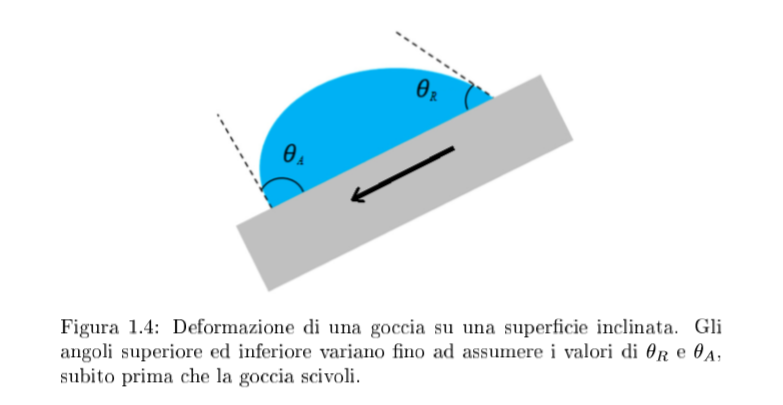
\includegraphics[width=0.8\columnwidth]{pinning.PNG}
	\label{fig:2}
\end{figure}
\subsection{Viscosità}
La viscosità descrive la resistenza di un materiale allo scorrimento (sforzo di taglio) ed ha le dimensioni di una pressione per un tempo.
Essa è una proprietà intrinseca che governa il moto dei fluidi e si indica con $\eta$. Vediamo come si può definire introducendo prima gamma dot, il gradiente  (stazionario) di velocità nello strato liquido, detto shear rate $\dot{\gamma} = \frac{\partial v}{\partial z}$ provocato a causa di uno sforzo di taglio (shear stress) $\sigma=\frac{F}{S}$ applicato alla superficie. La costante di proporzionalità tra le due grandezze
reologiche è proprio il coeffciente di viscosità: lo shear rate sarà tanto maggiore quanto maggiore è lo sforzo di taglio applicato.
\begin{equation}
\sigma=\eta\dot{\gamma}
\end{equation} 
\textbf{I fluidi per i quali $\eta$ è costante sono detti newtoniani} e sono caratterizzati da una rappresentazione sul piano $\sigma-\dot{\gamma}$ completamente lineare. \\
Esistono tuttavia anche casi, e sono i più comuni, nei quali la risposta allo sforzo di taglio non è lineare e, di conseguenza, la $\eta$ presenta una dipendenza ulteriore da $\gamma$:
\begin{equation}
\sigma=\eta(\dot{\gamma})\dot{\gamma}.
\end{equation} 
Questo comportamento identifica una vastissima categoria di fluidi, detti
appunto\textbf{ fluidi non-newtoniani, per i quali la viscosità varia con lo shear
rate}. Si classificano in questo ambito tre categorie di fluidi: shear
thinning, shear thickening e Bingham (fig. \ref{fig:3}).
\begin{figure}[h!] 
	\centering 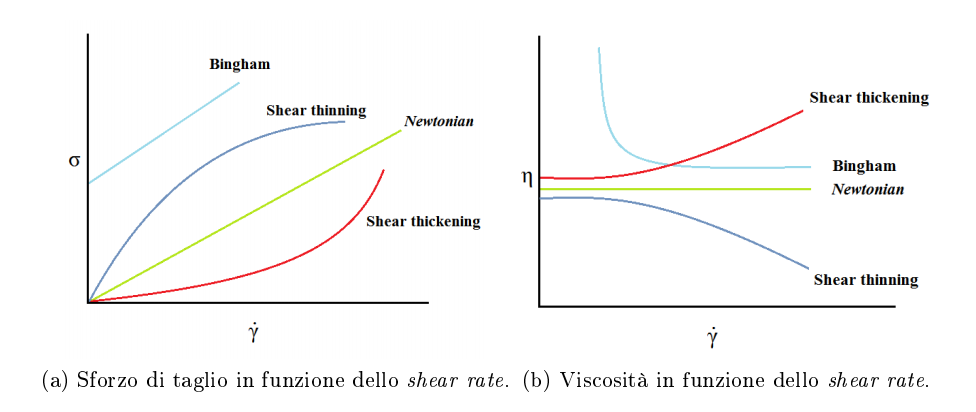
\includegraphics[width=1\columnwidth]{Nonnewtoniani.PNG}
	\label{fig:3}
\end{figure}

\subsection{Reologia}
La reologia è lo studio del fluire e del deformarsi di materiali sotto l'azione di forze esterne. Le proprietà reologiche possono essere misurate per sostanze che hanno struttura complessa, ad esempio per sospensioni, polimeri, composti del vetro( ad esempio silicati) ma anche molti cibi e additivi, fluidi corporei (es. il sangue) o altri materiali che appartengono alla classe della materia soffice.\\
In base a come la materia soffice risponde allo stress applicato, possiamo suddividerla in due grandi categorie: Newtoniani e Non-Newtoniani.

\subsubsection{Shear thinning}
Per i \textbf{fluidi pseudoplastici} o shear thinning la viscosità diminuisce all'aumentare dello shear rate: essi divengono in sostanza più fluidi all'aumentare dello stress applicato e per questo sono detti anche fluidi reofluidificanti.\\
A questa famiglia appartengono generalmente le dispersioni di polimeri a catena lineare: le molecole si trovano a riposo altamente aggrovigliate e tendono a disintrecciarsi all'aumentare dello stress, seguendo la direzione dello stesso, col risultato di migliorare lo scorrimento, ovvero di diminuire la viscosità.\\
Appartengono a questa categoria il sangue, molte soluzioni di biopolimeri e
un gran numero di liquidi d'uso industriale come vernici, schiume e adesivi.

\subsubsection{Shear thickening}
Nei \textbf{fluidi dilatanti} o shear thickening, al contrario dei precedenti, la viscosità aumenta all'aumentare della velocità di taglio e per questa ragione sono detti anche fluidi reoispessenti.\\
Si osserva questo tipo di comportamento sia in sospensioni colloidali (le particelle in sospensione tendono ad agglomerare, opponendosi allo scorrimento, con conseguente aumento di viscosità) che in soluzioni di biopolimeri particolarmente lunghi e ramificati (il tempo caratteristico di svolgimento del reticolo di macromolecole domina i tempi di scorrimento). Un noto esempio di fluido shear thickening è rappresentato dalle soluzioni di amido di mais in acqua.

\subsubsection{fluidi alla Bingham}
I sistemi caratterizzati da comportamento newtoniano al di sopra di uno
sforzo di soglia (quindi solo shiftati), cioè da una dipendenza del tipo:
\begin{equation}
\sigma=\eta\dot{\gamma}	+ \sigma_0
\end{equation}
sono chiamati fluidi viscoplastici o alla Bingham. Tali materiali iniziano a
comportarsi come un fluido solo dopo il superamento di una soglia di scorrimento (yield stress). Questo tipo di comportamento deriva dalla struttura reticolare generalmente posseduta da questi sistemi, che viene meno nel momento in cui si producano delle sollecitazioni uguali o superiori al limite di scorrimento. Il fenomeno della plasticità può risultare reversibile o meno a seconda che la struttura reticolare possa essere recuperata o meno.\\
Esempi di sistemi viscoplastici sono il ketchup, molti tipi di creme, gel o
unguenti.

\section{Studio dello scorrimento di gocce in seguito a sollecitazioni}
L'affnarsi delle tecniche applicate in reologia, ossia nello studio dello
scorrimento dei fluidi in seguito a sollecitazioni, ha permesso negli anni una ampia classificazione dei fluidi oggi conosciuti, sia naturali che artificiali.\\
Risulta oggi noto, così, come la maggior parte dei liquidi, ed in special modo i fluidi biologici, siano non-newtoniani e presentino, nella quasi totalità dei casi, comportamenti intermedi tra quelli tipici delle categorie poc'anzi elencate o li compendino in diverse zone di shear rate. Lo studio dei fluidi complessi acquisisce dunque importanza crescente sia nella ricerca di base che nelle applicazioni microbiologiche, mediche, alimentari e
industriali.
\subsection{Gocce su substrati oscillanti}

slide2
In queste condizioni il comportamento di un fluido è radicalmente diverso da quello che esprime a volumi ordinari perché caratterizzato dai fenomeni interfacciali e viscosi: le forze capillari dominano la gravità

Microfluidica aperta:

Numeri di Bond (Bo circa $10^{-12}$) è il rapporto tra la gravità e la tensione superficiale
numero reynolds:rapporto tra le forze d'inerzia e quelle viscose
g=acc. gravità
L=una lunghezza caratteristica del fenomeno considerato (ad esempio nel caso del moto di un fluido in una tubazione corrisponde al diametro del tubo, mentre nel caso di un profilo alare corrisponde alla lunghezza della corda
v=velocità di spostamento
rho=densità

slide 3
In presenza di una separazione tra due fluidi immiscibili (come ad esempio acqua e aria) le molecole poste all'interfaccia risentono di un sostanziale sbilanciamento di forze rispetto a quelle situate all'interno.
All'aumentare della superficie aumenta il numero di interazioni molecolari non bilanciate e quindi l'energia (libera) ad esse associata. Per espandere la superficie (A) è pertanto necessario fornire lavoro (W). Equivalentemente, la tensione superficiale si può interpretare come la forza per unità di lunghezza L che il fluido esercita perpendicolarmente ad ogni sezione dell'interfaccia (forza capillare).

la forma di una goccia sessile dipende unicamente dall'equilibrio fra le tensioni cui sono soggette le tre interfacce esistenti: quella tra substrato solido e liquido ($\gamma_{SL}$), quella tra solido e ambiente gassoso ($\gamma_{SG}$) e la tensione superficiale del liquido in aria ($\gamma$) dianzi presentata. 
leggere la disuguaglianza:
dispendio energetico per la formazione di un'interfaccia solido-liquido ed un'interfaccia liquido-vapore fosse inferiore a quello richiesto per formare un'area di separazione solido-vapore 

side 4
l'angolo di cont. è definito dalla leggge di Young e dipende dalla composizione della goccia e dalla comp. del substrato.
In base ad esso il fluido ha un comportamento diverso.

slide 5
Per poter definire la viscosità si devono prima definire shear rate e shear stress. Il primo è gamma dot, ossia il gradiente (stazionario) di velocità nello strato liquido,  provocato a causa di uno sforzo di taglio (shear stress) $\sigma=\frac{F}{S}$ applicato alla superficie.
La costante di proporzionalità tra le due grandezze
reologiche è il coeffciente di viscosità.

slide 6

oppure per sintetizzare: La goccia sessile SI COMPORTA COME UN'OSCILLATORE.
Una goccia sessile se messa in oscillazione attraverso un supporto meccanico od un semplice "soffio", manifesta comportamente armonici dovuti all'incomprimibilità del volume di un liquido e l'elasticità della sua superficie.
Questo perchè la tensione superficiale del liquido agisce da forza di richiamo verso la forma di equilibrio e permette un comportamento elastico dell'interfaccia, sulla quale si instaurano e trasmettono perturbazioni stazionarie. La goccia si trova in risonanza con la forzante e la frequenza di oscillazione coincide con un'autofrequenza nello spettro delle onde stazionarie sull'interfaccia per via del pinning della linea di contatto.

Sono stati studiati soprattutto recentemente queste oscillazioni. Nel nostro caso si possono considerare le oscillazioni verticali, poichè per avere oscillazioni orizzontali (ossia oscillazioni parallele al substrato e normali alla gravità), il centro di massa della goccia sessile oscilla orizzontalmente, provocando una variazione periodica degli angoli di contatto. Nel nostro caso non si hanno considerevoli variazioni del centro di massa come si può vedere dai video di seguito, in quanto siamo a volumi piuttosto alti per manifestarsi.

Il fattore alpha è un fattore trovato empiricamente, attribuito a fattori geometrici che poi recupera temperton (li incorpora in h).

slide 7
Lo scopo dell'esperienza è riprodurre il funzionamento di un reometro, un dispositivo che vediamo in figura in grado di applicare degli sforzi di taglio in direzioni diverse al liquido immesso e studiarne la reologia (quindi viscostà, tensione superficiale..). Lo si vuol fare a causa del fatto che serve una grande quantità di fluido e perchè è molto costoso quindi un'alternativa può essere (descrizione breve).
 
 
slide 9
Il segnale camptato rappresenta un segnale di voltaggio amplificato per poter essere acquisito, che mostra l'andamento periodico dell'oscillazione che va smorzandosi con il tempo. La differenza è immediata e sostanziale fra acqua up e il glicerolo 85\% che sappiamo avere viscosità 100 volte più alta.
slide 10
ho messo i video per far capire l'utilità della telecamera: si può osservare l'evaporazione della goccia, da questi video ricavo dei frame per poter poi calcorare su imagej l'arco L e la sua variazione, posso accorgermi se accadono fenomeni di depinnamento che mi causano errori nella misura.
slide 13
Per far vedere se si depinna che succede e per far vedere come ho deciso il sample rate e il nunero di samples, essendo che per samples più bassi si avevano meno punti (1000 hz e 8000 samples)

slide 14
a quanto pare i dati sono molto in accordo a meno di una leggera discrepanza per volumi più grandi, probablmente perchè le considerazioni geometriche non sussistono più. Invece notiamo una leggera discrepanza per il valore di volume più basso ($V=2 \mu L$) probabilmente perchè eravamo a fondo scala.

Si è fatta un'analisi per volumi più piccoli, Tale analisi è stata effettuata a causa del fatto che per volumi
 fra I 20 e I 100 si è notato una consistenza con il valore sperimentale
solo nel caso del primo modo d'oscillazione. Si attribuì così ciò 
al fatto che il modello potesse essere sbagliato per goccie con 
diametro maggiore della lunghezza di capillarità. Questo quindi porta all'analisi
di volumi più piccoli, essendo che questo limite è superato sin da subito
ossia fra 10 muL e 20 muL.
Da questa analisi però si evince che non si riesce ad osservare I modi successivi al primo, questo perchè le goccie sono troppo piccole per far sì che il laser catturi I modi successivi.

slide 15 
circa tutti consistenti a parte per due casi in cui uno la statistica è troppo povera, l'altro c'è sicuramente un errore legato al fatto che 20muL è il fondoscala della pipetta con cui ho preso i liquidi.
o forse perchè è molto viscoso con volumi molto piccoli quindi oscillano poco ed è più difficile fare la misura.

slide 16
esempi di gly + acqua, da notare come precedentemende detto che per volumi olto alti on si visualizzano picchi più bassi a causa del segnale sporco. Ho provato a sottrarre il fondo con il rumore di fondo ma non risolveva la situazione. In ogni caso succede che si visualizzano picchi più alti (esempio del V=70 del gly+ acqua al 60\%).
 In base a come soffiavo visualizzavo più o meno picchi, in base alla viscosità della goccia e alla grandezza visualizzavo picchi.
 ad esempio per l'acqua (viscosità bassa) visualizzavo molto bene tutto anche a volumi bassi, mentre avevo difficoltà a volumi più alti. per il glicerolo invece, più la viscosità era alta più era compicato visualizzare il primo modo per volumi bassi.
 
 slide 18
 setup 2 - serve a studiare le altre cose: sudio dell'angolo di contatto di acqua sul teflon, studia anche dell'isteresi dell'angolo e differenza con il parafilm per prendere confidenza con la teoria. Studio volto alla misurazione dell'angolo di contatto per le frequenze con acqua e glyceroli con teflon.
 Al fine di poter affinare gli errori ho fatto pure uno studio sulla variabilità della massa delle gocce, pesando più e più volte varie goccie dello stesso peso.
 
 slide viscosità e tensione superficiale
 Ho scelto la formula di Temperton perchè entrambe risultavano più o meno consistenti, ma la f. di Temperton è più precisa a livello di geometria con cui è stata calcolata, perchè si tiene conto del parametro h=altezza della goccia. Dunque è più accurata a volumi più alti e viscosità più alte. 
 
 conclusioni
 l'idea in un ambito più ampio è quella di misurare la reologia di una goccia sessile, questo è il primo step nel caso di fluidi newtoniani, in cui l'elasticità è data solo dal contributo capillare e non gravità. Nel caso di acqua e glicerolo usando il primo modo si trovano circa in accordo ma comunque la statistica è bassa. visto le varie difficoltà si può migliorare il metodo di oscillazione dell'eccitazione, usare substrati molto idrofobici (usare substrati impregnati con olio, che però abbasserebbero l'isteresi) e poi utilizzare liquidi viscoelastici.
 
 
 
\end{document}
